%
% File naaclhlt2018.tex
%
%% Based on the style files for NAACL-HLT 2018, which were
%% Based on the style files for ACL-2015, with some improvements
%%  taken from the NAACL-2016 style
%% Based on the style files for ACL-2014, which were, in turn,
%% based on ACL-2013, ACL-2012, ACL-2011, ACL-2010, ACL-IJCNLP-2009,
%% EACL-2009, IJCNLP-2008...
%% Based on the style files for EACL 2006 by 
%%e.agirre@ehu.es or Sergi.Balari@uab.es
%% and that of ACL 08 by Joakim Nivre and Noah Smith

\documentclass[11pt,a4paper]{article}
\usepackage[hyperref]{emnlp2018}
% \usepackage[showframe=true]{geometry}
\usepackage[utf8]{inputenc}
\usepackage{times}
\usepackage{latexsym}
\usepackage{lipsum}
\usepackage{url}
\usepackage{multirow}
\usepackage{changepage}
\usepackage{amssymb}
\usepackage{bm}
\usepackage{amsmath}
\usepackage{graphicx}
\usepackage{siunitx}
\usepackage[hang,flushmargin]{footmisc} % remove indentation from footnotes
% \hypersetup{draft}

\aclfinalcopy % Uncomment this line for the final submission
%\def\aclpaperid{***} %  Enter the acl Paper ID here

%\setlength\titlebox{5cm}
% You can expand the titlebox if you need extra space
% to show all the authors. Please do not make the titlebox
% smaller than 5cm (the original size); we will check this
% in the camera-ready version and ask you to change it back.

\newcommand\BibTeX{B{\sc ib}\TeX}
\newcommand\confname{EMNLP 2018}
\newcommand\conforg{SIGDAT}
\newcommand{\colrule}{\noindent\rule{8cm}{0.4pt}}
\newcommand{\colruleend}{\noindent\rule{8cm}{2.0pt}}

% Avoid breaking inline equations ALWAYS (might break layout)
% https://tex.stackexchange.com/questions/14241/how-can-i-prevent-latex-from-breaking-inline-formulas-globally
\relpenalty=10000
\binoppenalty=10000


\title{IIIDYT at IEST 2018: Implicit Emotion Classification With Deep
Contextualized Word Representations}

\author{Jorge A. Balazs, Edison Marrese-Taylor \and Yutaka Matsuo \\
  Graduate School of Engineering\\
  The University of Tokyo\\
  {jorge, emarrese, matsuo@weblab.t.u-tokyo.ac.jp} \\
}

\date{}

% Style for acronyms; avoids splitting them.
% See https://tex.stackexchange.com/questions/48435/how-do-i-prevent-tex-from-hyphenating-acronyms
\newcommand{\Acronym}[1]{\mbox{#1}}

\begin{document}
\maketitle
\begin{abstract}
In this paper we describe our system designed for the WASSA 2018 Implicit Emotion Shared Task (IEST), which obtained 2$^{\text{nd}}$ place out of 26 teams with a test macro F1 score of $0.710$. The system is composed of a single pre-trained ELMo layer for encoding words, a Bidirectional Long-Short Memory Network BiLSTM for enriching word representations with context, a max-pooling operation for creating sentence representations from said word vectors, and a Dense Layer for projecting the sentence representations into label space. Our official submission was obtained by ensembling 6 of these models initialized with different random seeds.
\end{abstract}

\section{Introduction}

Although the definition of emotion is still debated among the scientific community, the automatic identification and understanding of human emotions by machines has long been of interest in computer science. It has usually been assumed that emotions are triggered by the interpretation of a stimulus event according to its meaning. 

As language usually reflects the emotional state of an individual, it is natural to study human emotions by understanding how they are reflected in text. We see that many words indeed have affect as a core part of their meaning, for example, \textit{dejected} and \textit{wistful} denote some amount of sadness, and are thus associated with sadness. On the other hand, some words are associated with affect even though they do not denote affect. For example, \textit{failure} and \textit{death} describe concepts that are usually accompanied by sadness and thus they denote some amount of sadness. In this context, the task of automatically recognizing emotions from text has recently attracted the attention of researchers in Natural Language Processing. This task is usually formalized as the classification of words, phrases, or documents into predefined discrete emotion categories or dimensions. Some approaches have aimed at also predicting the degree to which an emotion is expressed in text \cite{wassa_emoint_2017}.

In light of this, the \Acronym{WASSA} 2018 Implicit Emotion Shared Task (\Acronym{IEST}) \cite{klinger2018iest} was proposed to help find ways to automatically learn the link between situations and the emotion they trigger. The task consisted in predicting the emotion of a word excluded from a tweet. Removed words, or \textit{trigger-words}, included the terms ``sad'', ``happy'', ``disgusted'', ``surprised'', ``angry'', ``afraid'' and their synonyms, and the task was to predict the emotion they conveyed, specifically sadness, joy, disgust, surprise, anger and fear.

From a machine learning perspective, this problem can be seen as sentence classification, in which the goal is to classify a sentence, or in particular a tweet, into one of several categories. In the case of \Acronym{IEST}, the problem is specially challenging since tweets contain informal language, the heavy usage of emoji, hashtags and username mentions.

In this paper we describe our system designed for \Acronym{IEST}, which obtained the second place out of 26 teams. Our system did not require manual feature engineering and only minimal use of external data. Concretely, our approach is composed of a single pre-trained \Acronym{ELMo} layer for encoding words \cite{peters2018deep}, a Bidirectional Long-Short Memory Network (\Acronym{BiLSTM}) \cite{graves2005framewise, graves2013speech}, for enriching word representations with context, a max-pooling operation for creating sentence representations from said word vectors, and finally a Dense Layer for projecting the sentence representations into label space. To the best of our knowledge, our system, which we plan to release, is the first to utilize ELMo for emotion recognition. 


%  \item Code will be made available

% FIXME: EDIT THIS SECTION TO MAKE PARAGRAPHS MORE COHESIVE
% Sentiment Analysis, also known as Opinion Mining, is a discipline whose
% objective is to automatically identify sentiment in written text
% \cite{balazs2016opinion}.

\begin{figure*}
    \centering
    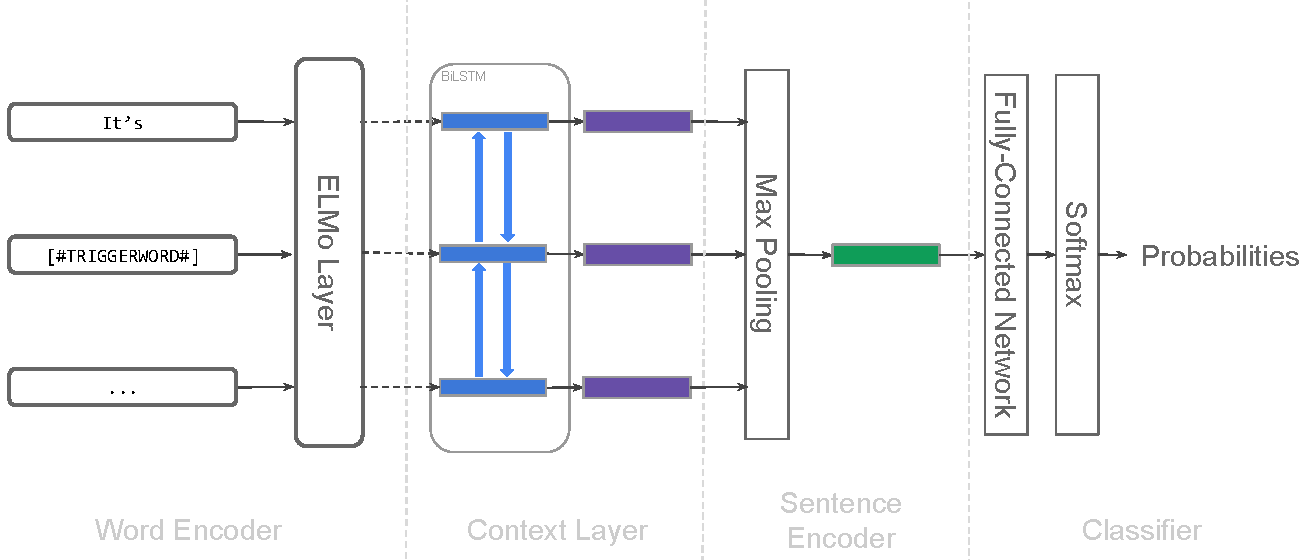
\includegraphics[scale=0.6]{images/iest_architecture.pdf}
    \caption{Proposed architecture.}
    \label{fig:architecture}
\end{figure*}

\section{Proposed Approach}

\subsection{Preprocessing}

As our model is purely character-based, we performed little data preprocessing. Table \ref{table:substitutions} shows the special tokens found in the datasets, and how we substituted them. 

\begin{table}[!h]
    \centering
    \footnotesize

    \begin{tabular}{ll}

        \textbf{Original} & \textbf{Replacement} \\
        \hline
        \hline
        \texttt{\footnotesize[\#TRIGGERWORD\#]} & \texttt{\footnotesize\_\_TRIGGERWORD\_\_} \\
        \texttt{\footnotesize@USERNAME} & \texttt{\footnotesize\_\_USERNAME\_\_} \\
        \texttt{\footnotesize[NEWLINE]} & \texttt{\footnotesize\_\_NEWLINE\_\_} \\
        \texttt{\footnotesize http://url.removed} & \texttt{\footnotesize\_\_URL\_\_} \\

    \end{tabular}
    \caption{Preprocessing substitutions.}
    \label{table:substitutions}
\end{table}

    Furthermore, we tokenized the text using a variation of the
    \texttt{twokenize.py}\footnote{\tiny\url{https://github.com/myleott/ark-twokenize-py}}
    script, a Python port of the original \texttt{Twokenize.java}
    \cite{gimpel-EtAl:2011:ACL-HLT2011}. Concretely, we created an emoji-aware
    version of it by incorporating knowledge from an emoji
    database,\footnote{\tiny\url{https://github.com/carpedm20/emoji/blob/e7bff32/emoji/unicode_codes.py}}
    which we slightly modified for avoiding conflict with emoji sharing unicode
    codes with common glyphs used in Twitter,\footnote{For example, the hashtag
    emoji is composed by the unicode code points \texttt{U+23 U+FE0F U+20E3},
which include \texttt{U+23}, the same code point for the \texttt{\#} glyph.} and for making it compatible with Python 3.
% \begin{itemize}
%     \item briefly describe previous Semeval papers~\cite{baziotis2018ntua,
%         duppada2018seernet, abdou2018affecthor} (Should we do this despite not
%         having based our work in any of them?)
%     \item mention previous Wassa papers
%     \item talk about some sentence classification tasks? Works that fall into
%         the broad category of mapping sentences to labels.
%     \item Talk about elmo~\cite{peters2018deep}
% \end{itemize}

\subsection{Architecture}

Figure \ref{fig:architecture} summarizes our proposed architecture. Our input is based on Embeddings from Language Models (ELMo) by \citet{peters2018deep}. These are character-based word representations allowing the model to avoid the ``unknown token'' problem. ELMo uses a set of convolutional neural networks to extract features from character embeddings, and builds word vectors from them. These are then fed to a multi-layer Bidirectional Language Model (BiLM) which returns context-sensitive vectors for each input word. 

We used a single-layer BiLSTM as context fine-tuner \cite{graves2005framewise, graves2013speech}, on top of the ELMo embeddings, and then aggregated the hidden states it returned by using max-pooling, which has been shown to perform well on sentence classification tasks \cite{conneau2017supervised}.

Finally, we used a single-layer fully-connected network for projecting the pooled BiLSTM output into a vector corresponding to the label logits for each predicted class.

\subsection{Implementation Details and Hyperparameters}

\hspace{\parindent} \textbf{ELMo Layer}: We used the official AllenNLP implementation of the ELMo model\footnote{\tiny\url{https://allenai.github.io/allennlp-docs/api/allennlp.modules.elmo.html}}, with the official weights pre-trained on the 1 Billion Word Language Model Benchmark, which contains about 800M tokens of news crawl data from WMT 2011 \cite{Chelba2014}.

\textbf{Dimensionalities}: By default the ELMo layer outputs a 2048-dim vector, which we then feed to a BiLSTM resulting in a 4096-dim vector for each word of the sequence\footnote{A BiLSTM is composed of two separate LSTMs that read the input in opposite directions and whose outputs are concatenated at the sequence dimension. This results in a vector double the dimension of the input for each time step.}. After max-pooling the BiLSTM output over the sequence dimension we have a single 4096-dim vector corresponding to the tweet representation. This representation is finally fed to a single-layer fully-connected network with input size 4096, 512 hidden units, output size 6, and ReLU nonlinearities after the input and hidden layers. The output of the dense layer is a 6-dim logit vector for each example.

\textbf{Loss Function}: As this corresponds to a multiclass classification problem (predicting a single class for each example, with more than 2 classes to choose from), we used the Cross-Entropy Loss as implemented in PyTorch \cite{paszke2017automatic}.

\textbf{Optimization}: We optimized the model with Adam \cite{DBLP:journals/corr/KingmaB14}, using a slanted triangular learning rate schedule \cite{howard2018universal}, with default hyperparameters ($cut\_frac=0.1$, $ratio=32$), and a maximum learning rate $\eta_{max}=0.001$, over $T=23,970$ iterations\footnote{This number is obtained by multiplying the number of epochs ($10$) times the total number of batches, which for the training dataset corresponds to $2396$ batches of $64$ elements, and $1$ batch of $39$ elements, hence $2397\times10=23,970$.}.

\textbf{Regularization}: we used a dropout layer \cite{srivastava2014dropout}, with probability of 0.5 after both the ELMo and the hidden fully-connected layer, and another one with probability of 0.1 after the max-pooling aggregation layer. We also reshuffled the training examples between epochs, resulting in a different batch for each iteration. 

\textbf{Model Selection}: To choose the best hyperparameter configuration we measured the classification accuracy on the validation set (trial set). 


\subsection{Ensembles}
 
Once we found the best-performing configuration we trained 10 models using different random seeds, and tried averaging the output probabilities of all their possible $\sum_{k=1}^{10}{\binom{10}{k}}=1023$ combinations. As Figure \ref{fig:best_ensembles} shows, we empirically found that a specific combination of $6$ models yielded the best results ($70.52\%$), providing evidence for the fact that using a number of independent classifiers equal to the number of class labels provides the best results when doing average ensembling \cite{bonab2016theoretical}.


\begin{figure}[!h]
    \centering
    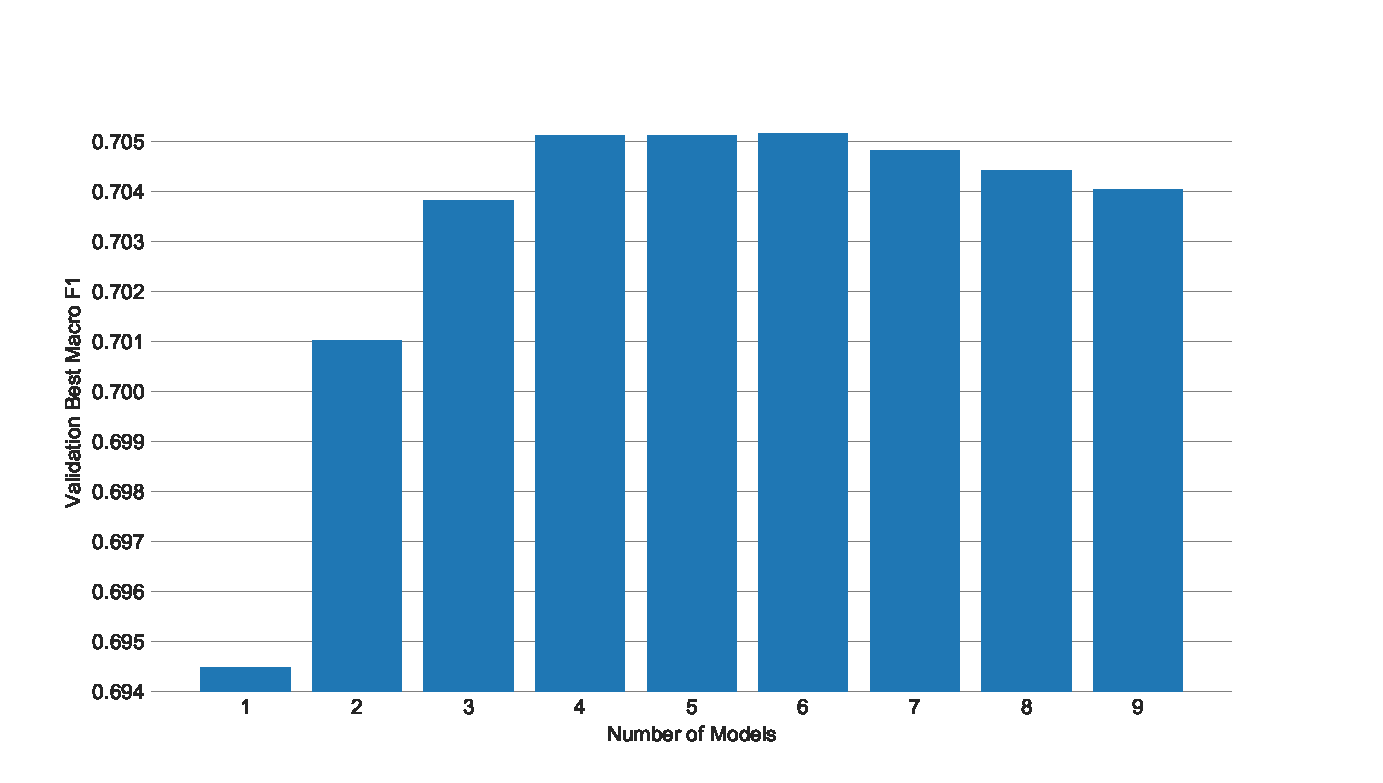
\includegraphics[width=\columnwidth]{images/best_ensembles.eps}
\caption{Best Macro F1 vs. Number of Ensembled Models.}
\label{fig:best_ensembles}
\end{figure}

\section{Experiments and Analyses}

We performed several experiments to gain insights on how the proposed model's performance interacts with the shared task's data. We performed an ablation study to see how some of the main hyperparameters affect performance, and an analysis of tweets containing hashtags and emoji to understand how these two types of tokens help the model predict the trigger-word's emotion. We also observed the effects of varying the amount of data used for training the model to evaluate whether it would be worthwhile to gather more training data.

\subsection{Ablation Study}%
\label{sub:ablation_study}

We performed an ablation study on a single model having obtained 69.23\% accuracy on the validation set. Results are summarized in Table \ref{table:ablation}.

\begin{table}[!h]
    \centering
    \footnotesize

    \begin{tabular}{lcc}

        \textbf{Variation} & \textbf{Accuracy (\%)} & $\bf{\Delta}$\textbf{\%} \\
        \hline
        \hline
        Submitted          & \textbf{69.23}         & -                        \\
        \hline
        No emoji           & 68.36                  & - 0.87                   \\
        \hline
        No ELMo            & 65.52                  & - 3.71                   \\
        \hline
        Concat Pooling     & 68.47                  & - 0.76                   \\
        \hline
        LSTM hidden=4096   & 69.10                  & - 0.13                   \\
        LSTM hidden=1024   & 68.93                  & - 0.30                   \\
        LSTM hidden=512    & 68.43                  & - 0.80                   \\
        \hline
        POS emb dim=100    & 68.99                  & - 0.24                   \\
        POS emb dim=75     & 68.61                  & - 0.62                   \\
        POS emb dim=50     & 69.33                  & + 0.10                   \\
        POS emb dim=25     & 69.21                  & - 0.02                   \\
        \hline
        SGD optim lr=1     & 64.33                  & - 4.90                   \\
        SGD optim lr=0.1   & 66.11                  & - 3.12                   \\
        SGD optim lr=0.01  & 60.72                  & - 8.51                   \\
        SGD optim lr=0.001 & 30.49                  & - 38.74                  \\

    \end{tabular}
    \caption{Ablation study results.}
    \label{table:ablation}

\end{table}

Accuracies were obtained from the
validation dataset. Each model was trained with the same random seed and hyperparameters, save for the one listed. ``No emoji'' is the same model trained on the training dataset with no emoji, ``No ELMo'' corresponds to having switched the ELMo word encoding layer with a simple pre-trained GloVe embedding lookup, and ``Concat Pooling'' obtained sentence representations by using the pooling method described by \citet{howard2018universal}. ``LSTM hidden'' corresponds to the the hidden dimension of the BiLSTM, ``POS emb dim'' to the dimension of the part-of-speech embeddings, and ``SGD optim lr'' to the learning rate used while optimizing with the schedule described by \citet{conneau2017supervised}.

We can observe that the architectural choice that had the greatest impact on our model was the ELMo layer, providing a $3.71\%$ boost in performance as compared to using GloVe pre-trained word embeddings.

We can further see that emoji also contributed significantly to the model's performance. In Section \ref{sub:effect_of_emoji_and_hashtags} we give some pointers to understanding why this is so.  

Additionally, we tried using the concatenation of the max-pooled, average-pooled and last hidden states of the BiLSTM as the sentence representation, following \citet{howard2018universal}, but found out that this impacted performance negatively. We hypothesize this is due to tweets being too short for needing such a rich representation. Also, the size of the concatenated vector was $4096\times3=12,288$, which probably could not be properly exploited by the 512-dimensional fully-connected layer.

Using a greater BiLSTM hidden size did not help the model, probably because of the reason mentioned early; the fully-connected layer was not big or deep enough to exploit the additional information. Similarly, using a smaller hidden size neither helped.

We found that using 50-dim part-of-speech embeddings slightly improved results, which implies that better fine-tuning this hyperparameter, or using a better POS tagger could yield an even better performance.

Regarding optimization strategies, we also tried using SGD with different learning rates and a step-wise learning rate schedule as described by \citet{conneau2018}, but we found that doing this did not improve performance. 

Finally, Figure \ref{fig:dropouts} shows the effect of using different dropout probabilities. We can see that having higher dropout after the word-representation layer and the fully-connected network's hidden layer, while having a low dropout after the sentence encoding layer yielded better results overall. 

\begin{figure}[!h]
    \centering
    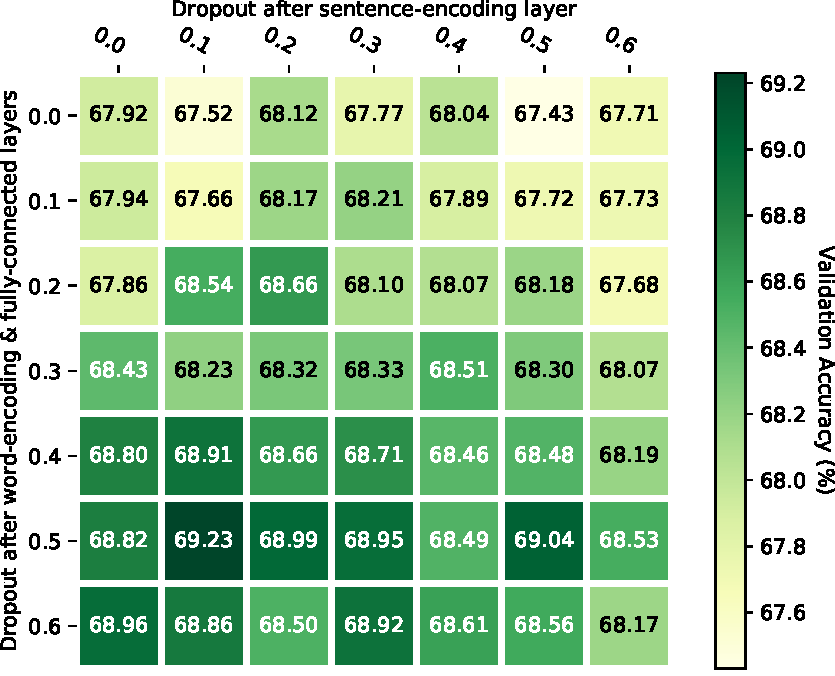
\includegraphics[width=\columnwidth]{images/dropout_table.pdf}
\caption{Dropout Variations. Rows correspond to the dropout applied both after the ELMo layer (word encoding layer) and after the fully-connected network's hidden layer, while columns correspond to the dropout applied after the max-pooling operation (sentence encoding layer.}
\label{fig:dropouts}
\end{figure}

\subsection{Effect of Emoji and Hashtags}%
\label{sub:effect_of_emoji_and_hashtags}

\begin{table}[!h]
    \centering
    \footnotesize

    \begin{tabular}{lcc}

        \textbf{} & \textbf{Present} & \textbf{Not Present} \\
        \hline
        \hline
        Emoji     & 4805 (76.6\%)    & 23952 (68.0\%)       \\
        Hashtags  & 2122 (70.5\%)    & 26635 (69.4\%)       \\

    \end{tabular}

    \caption{Number of tweets on the test set with and without emoji and
    hashtags. The number between parentheses is the proportion of tweets
    correctly classified.}

    \label{table:emoji_and_hashtags}

\end{table}

Table \ref{table:emoji_and_hashtags} shows the overall effect of hashtags and
emoji on classification performance. Tweets containing emoji seem to be easier
for the model to classify than those without. Hashtags also have a positive
effect on classification performance, however it is less significant. This implies that emoji, and hashtags in a smaller degree, provide
tweets with a context richer in sentiment information, allowing the model to
better guess the emotion of the \textit{trigger-word}.

Table \ref{table:emoji_fine_grained} shows the effect specific emoji have on classification performance. 

\begin{table}[!h]
    \centering
    \scriptsize
        \begin{tabular}{lr|rc|rc|r}

           \multirow{2}{*}{\textbf{Emoji alias}} & \multirow{2}{*}{\textbf{N}} & \multicolumn{2}{c|}{\textbf{emoji}} & \multicolumn{2}{c|}{\textbf{no-emoji}} &
            \multirow{2}{*}{$\bf{\Delta}$\textbf{\%}} \\
            \cline{3-6}
                                &     & \#   & \% & \# & \% & \\
          \hline
          \hline
          \texttt{mask}         & 163 & 154 & 94.48 & 134 & 82.21 & - 12.27 \\
          \texttt{two\_hearts}  & 87  & 81  & 93.10 & 77  & 88.51 & - 4.59  \\
          \texttt{heart\_eyes}  & 122 & 109 & 89.34 & 103 & 84.43 & - 4.91  \\
          \texttt{heart}        & 267 & 237 & 88.76 & 235 & 88.01 & - 0.75  \\
          \texttt{rage}         & 92  & 78  & 84.78 & 66  & 71.74 & - 13.04 \\
          \texttt{cry}          & 116 & 97  & 83.62 & 83  & 71.55 & - 12.07 \\
          \texttt{sob}          & 490 & 363 & 74.08 & 345 & 70.41 & - 3.67  \\
          \texttt{unamused}     & 167 & 121 & 72.46 & 116 & 69.46 & - 3.00  \\
          \texttt{weary}        & 204 & 140 & 68.63 & 139 & 68.14 & - 0.49  \\
          \texttt{joy}          & 978 & 649 & 66.36 & 629 & 64.31 & - 2.05  \\
          \texttt{sweat\_smile} & 111 & 73  & 65.77 & 75  & 67.57 & 1.80 \\
          \texttt{confused}     & 77  & 46  & 59.74 & 48  & 62.34 & 2.60 \\

        \end{tabular}


    \caption{Fine grained performance on tweets containing emoji, and the effect of removing them. \textbf{N} is the total number of tweets containing the listed emoji, \textbf{\#} and \textbf{\%} the number and percentage of correctly-classified tweets respectively, and $\bf{\Delta}$\textbf{\%} the variation of test accuracy when removing the emoji from the tweets.}

    \label{table:emoji_fine_grained}

\end{table}

It is clear some emoji strongly contribute to improving prediction quality. The most interesting ones are \texttt{mask}, \texttt{rage}, and \texttt{cry}, which significantly increase accuracy. Further, contrary to intuition, the \texttt{sob} emoji contributes less than \texttt{cry}, despite representing a stronger emotion. This is probably due to \texttt{sob} being used for depicting a wider spectrum of emotions.

Finally, not all emoji are beneficial for this task. When removing \texttt{sweat\_smile} and \texttt{confused} accuracy increased, probably because they represent emotions other than the ones being predicted.
%From observing Table \ref{table:emoji_label} it seems likely that tweets containing \texttt{mask} would be highly predictive of the \texttt{disgust} class, since more than $92\%$ of the tweets containing such emoji belong to that class, however it less clear why \texttt{rage}, and \texttt{cry} contribute similarly, despite being more evenly distributed among classes.

%This means that they are highly representative of the the class the tweet belongs to, and would be good choices for discriminating new tweets in case we wanted to expand the dataset.

%For example, by observing Table \ref{table:emoji_label} we can infer that  \texttt{mask}, \texttt{rage}, and \texttt{cry}   \texttt{disgust}, \texttt{rage}, and \texttt{sad} classes respectively.

\subsection{Effect of the Amount of Training Data}

As Figure \ref{fig:data_amt_vs_acc} shows, increasing the amount of data in which our model was trained consistently increased validation accuracy and validation macro F1 score. The trend shows that having more training data would likely further increase the model's performance.

\begin{figure}[!h]
    \centering
    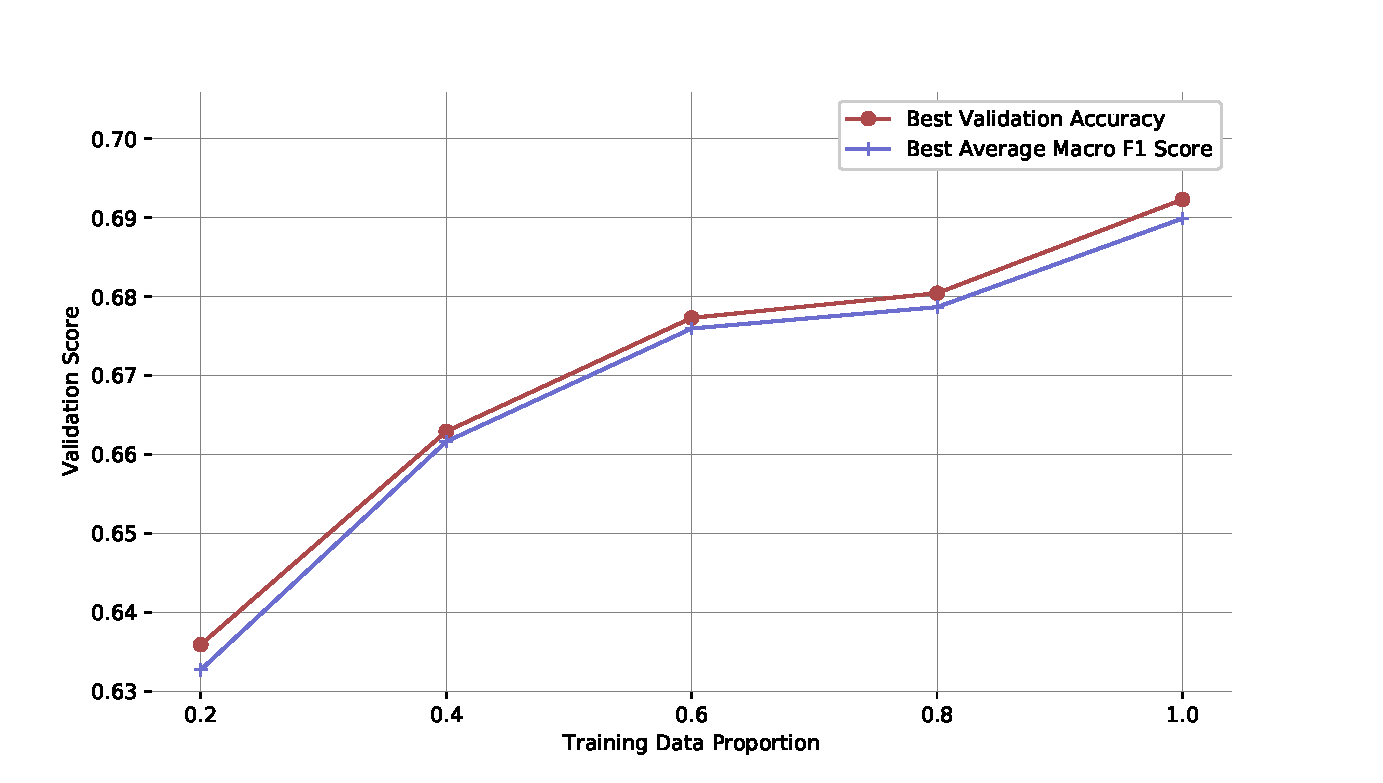
\includegraphics[width=\columnwidth]{images/acc_vs_tdp_variation.eps}
    \caption{Validation accuracy and macro F1 score vs. proportion of the training data.}
    \label{fig:data_amt_vs_acc}
\end{figure}

\section{Conclusions and Future Work}

We described the model that got second place in the WASSA 2018 Implicit Emotion Shared Task. Despite its simplicity, and low amount of dependencies on libraries and external features, it performed almost as well as the system that obtained the first place.

Our ablation study revealed that our hyperparameters were indeed quite well-tuned for the task, which agrees with the good results obtained in the official submission. However, the ablation study also showed that increased performance can be obtained by incorporating POS embeddings as additional inputs. Further experiments are required to accurately measure the impact that this additional input may have on the results. We also think the performance can be boosted by making the architecture more complex, concretely, by using a BiLSTM with multiple layers and skip connections in a way akin to \cite{peters2018deep}, or by making the fully-connected network bigger and deeper.

Finally, our studies regarding the importance of hashtags and emoji in the classification showed that both of them seem to contribute significantly to the performance, although in different measures. 

\bibliography{bibliography}
\bibliographystyle{acl_natbib_nourl}


\end{document}
